\documentclass{article}

\usepackage[T1]{fontenc}
\usepackage{indentfirst}
\usepackage{xcolor,graphicx,url}
\usepackage[utf8]{inputenc}
\usepackage{subfigure}
\usepackage{amsmath}
\usepackage[english,brazil]{babel} %hifenação em português e inglês
\usepackage{newcent} %fonte New Century
\usepackage{natbib}%% trabalha as referências bibliográficas
\usepackage{palatino, url, multicol}
\usepackage{listings}
\usepackage{lscape}
\usepackage{synttree}
\usepackage{pdfpages}



\begin{document}
\begin{sloppypar}
\everymath{\displaystyle}

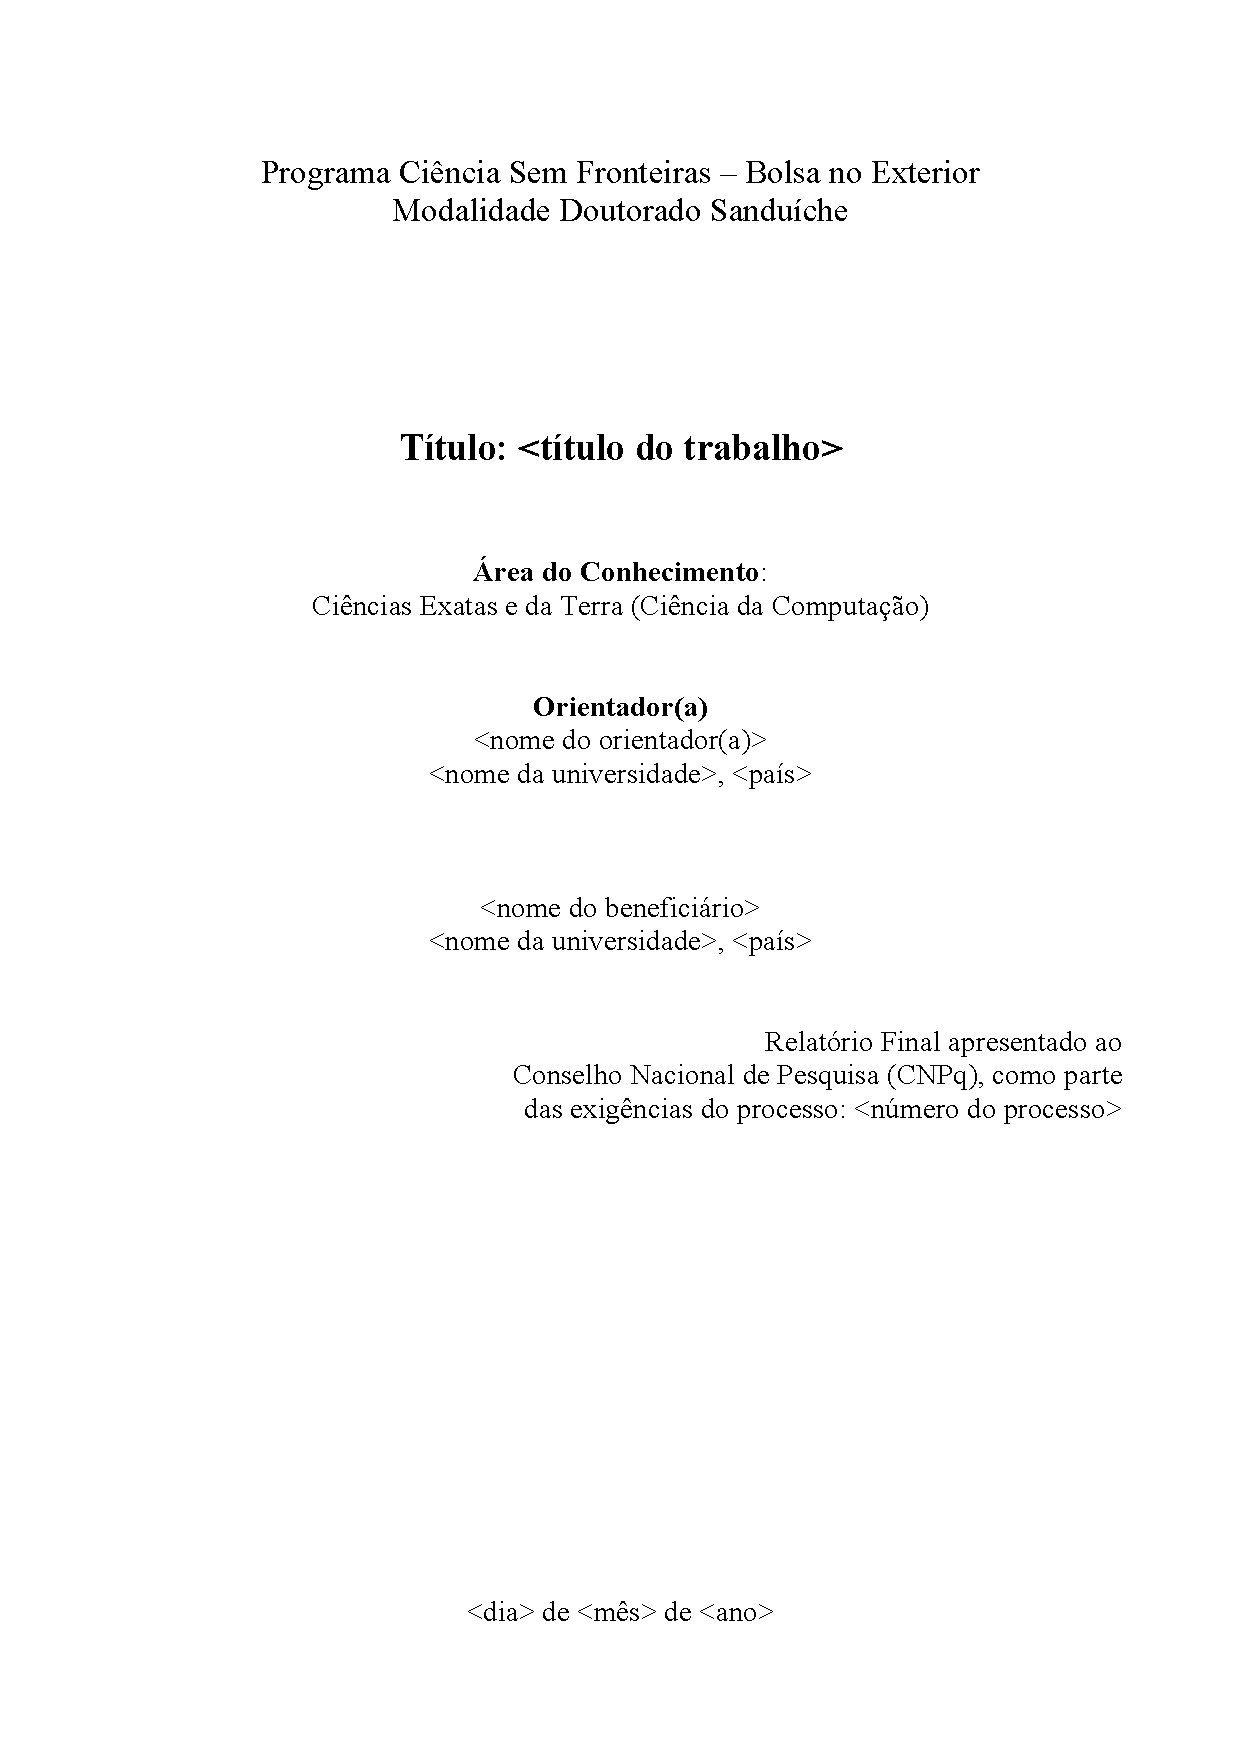
\includepdf[pages={1}]{00-pretextos/folha-rosto.pdf}

\section{Introdução e Motivação}\label{sec:introduction}

Introdução e motivação da pesquisa.\textbf{}
\section{Objetivos}\label{sec:goals}

\subsection{Objetivos da bolsa de doutorado sanduíche}

\subsection{Objetivos do doutorado}
\section{Metodologia}\label{sec:methodology}

\section{Conclusão}\label{sec:conclusao}




\footnotesize
\bibliographystyle{alpha}
\bibliography{03-references/references}

\normalsize
\section{Atividades desenvolvidas}\label{sec:atividades}

Descrever as principais atividades desenvolvidas/trabalhos executados. Caso o andamento das atividades não tenha transcorrido conforme o cronograma, esse fato deverá ser justificado.
\section{Publicações}\label{sec:publicacoes}

Se os trabalhos conduzidos geraram artigos para publicação em anais de congressos ou revistas especializadas, cópias destes devem ser incluídas na forma de anexos.

\subsubsection{Título do artigo 1}

%\includepdf{artigo_1}
Resumo do artigo 1

$\cdots$

\subsubsection{Título do artigo$_n$}

Resumo do artigo$_n$

%\includepdf{artigo_n}
\section{Outras atividades acadêmicas}\label{sec:outras-atividades}

\end{sloppypar}

\end{document}